% Scientific poster (A0) -- ctan:sciposter. Licence: NO grant text anywhere
% in the vendored sciposter.cls (checked directly, no README/doc bundled in
% the pinned TeX Live tree either) -- shipped as UNKNOWN per this batch's
% licence policy (no licence found anywhere -> ship it). Author per the class
% header comment: Michael H.F. Wilkinson and Alle Meije Wink. Ships with TeX
% Live -- starter does not bundle the class.
%
% sciposter is article-based with NO automatic multi-column layout (unlike
% baposter/tikzposter) -- \Section/\sSection key off \columnwidth, so the
% body must be wrapped in multicol itself, or the sections render full-width
% across the whole A0 sheet. \printleftlogo/\printrightlogo default to empty
% horizontal space (no bundled image needed) so the class's default
% useleftlogo/userightlogo=true is safe to leave on.
%
% PATCHED (latextemplates.com): two real failures found and fixed here.
% (1) An earlier draft compiled cleanly but rendered ONLY THE TOP THIRD of
% the A0 sheet -- the exact "fills only the top of the page" failure this
% batch was warned about, via multicol's default column-BALANCING (which
% shrinks to fit short content) rather than a stretch bug, compounded by a
% stray \vfill\null\columnbreak forcing an early column break. Fixed by
% removing the forced break and writing substantially more genuine content
% (Related Work, an extended Method, Discussion, System Architecture
% diagram, a second evaluation figure, an ablations table) so the three
% columns fill most of the page height on their own.
% (2) \centerline{...} on a multi-line figure/table caption does NOT add
% trailing vertical space and mis-measures multi-line text -- captions were
% overlapping the NEXT \Section box in the rendered preview, silently (no
% compile warning). Replaced every caption with center...end{center} +
% \medskip, which measures and spaces correctly.
\documentclass[a0,portrait,final]{sciposter}
\usepackage[utf8]{inputenc}
\usepackage[T1]{fontenc}
\usepackage{multicol}
\usepackage{graphicx}
\usepackage{booktabs}
\usepackage{tikz}
\usepackage{amsmath}

\title{Adaptive Caching Cuts Tail Latency by 41\% in Multi-Tenant Query Engines}
\author{A. Researcher$^1$, B. Collaborator$^1$, C. Advisor$^2$}
\renewcommand{\theinstitute}{$^1$Department of Computer Science, University of Somewhere \quad $^2$Data Systems Lab, Somewhere Institute of Technology}
\renewcommand{\printemail}{a.researcher@somewhere.edu}
\conference{ACM SIGMOD 2026}

\begin{document}
\maketitle

\begin{multicols}{3}

\Section{Abstract}
Multi-tenant query engines share cache space across workloads with very
different access patterns, and static eviction policies leave tail latency
at the mercy of whichever tenant last touched the cache. We introduce
\textsc{TenantLRU}, a per-tenant weighted caching scheme that adapts
eviction pressure to each tenant's observed hit-rate curve. Across three
production-scale traces, \textsc{TenantLRU} cuts p99 latency by 41\% and
p50 by 12\%, with under 2\% additional memory overhead.

\Section{Introduction}
Shared caches in multi-tenant systems face a well-known fairness problem:
a single global LRU policy optimises aggregate hit rate at the expense of
tenants whose access patterns do not fit the dominant working set. This is
especially visible under skewed load, where a handful of noisy tenants can
starve smaller ones of cache capacity entirely, inflating their tail
latency even though the system-wide hit rate looks healthy.

Prior work addresses this either by static partitioning (which wastes
capacity when tenants are idle) or by cost-based admission policies tuned
offline per workload. Neither adapts online to shifting tenant behaviour.
\textsc{TenantLRU} instead tracks a lightweight per-tenant miss-rate curve
and reallocates weighted cache shares every epoch, with no offline tuning
step and no per-workload configuration.

\Section{Related Work}
Miss-ratio-curve (MRC) estimation has a long history in cache research.
ARC~[1] adapts between recency and frequency online but assumes a
single tenant and a single policy for the whole cache. LHD~[2]
models hit density directly and generalises well across workloads, but its
per-object cost model is expensive to maintain per tenant at our scale.
SHARDS~[3] showed that spatial sampling makes MRC construction
cheap enough to run online, which is the piece we build on: rather than
one global MRC, \textsc{TenantLRU} maintains one cheap sampled MRC per
tenant and turns the allocation problem into a per-epoch knapsack solved
greedily. Cost-aware admission policies (e.g.\ TinyLFU-style filters) are
complementary — they decide what enters the cache, while
\textsc{TenantLRU} decides how much space each tenant is entitled to.

\Section{Method}
Each tenant $t$ maintains a sampled miss-rate curve $M_t(c)$ estimated via
a shadow LRU stack of size $c_{\max}$, refreshed continuously from a
uniformly sampled subset of that tenant's accesses (following the SHARDS
sampling scheme, at a 1-in-256 rate). Every epoch, we solve

\[
  \max_{\{c_t\}} \sum_t w_t \cdot (1 - M_t(c_t))
  \quad \text{s.t.} \quad \sum_t c_t \le C,
\]

\noindent where $w_t$ is a tenant priority weight and $C$ is total cache
capacity, using a greedy marginal-gain allocator that runs in
$O(T \log T)$ per epoch for $T$ tenants. Shadow stacks add under 2\% memory
overhead relative to the live cache.

The allocator re-solves the knapsack every epoch (default: every 30
seconds of wall-clock traffic, configurable), rather than continuously, to
keep the marginal-gain bookkeeping cheap: recomputing $M_t(c)$ for every
tenant on every cache access would dominate the hot path. Between epochs,
each tenant is enforced against its allocated share $c_t$ with a standard
LRU eviction order local to that tenant's partition — the global policy
only decides partition sizes, not eviction order within a partition, which
keeps the per-access cost identical to a plain LRU cache.

We additionally cap how much any single tenant's share can grow or shrink
in one epoch (a 20\% band by default), which damps oscillation when a
tenant's access pattern shifts abruptly — an unbounded reallocation policy
tended to overreact to short bursts in early experiments and produced
worse tail latency than a static split during bursty traffic.

\Section{Discussion}
Two design choices are worth calling out. First, weighting by $w_t$ rather
than giving every tenant an equal share means an operator can express
business priority directly, without hand-tuning static partition sizes —
in our production deployment $w_t$ is set from an existing per-tenant SLA
tier, so no new configuration surface was introduced. Second, solving the
allocation problem per epoch rather than continuously bounds the overhead
of the scheme to a small, predictable slice of total CPU time, which made
it easy to get sign-off for a production rollout: the worst case is a
bounded knapsack solve, not an unbounded per-access cost.

% PATCHED (latextemplates.com): this diagram originally used a wide
% horizontal layout (nodes spread across ~8.4 TikZ units) sized for a full
% poster WIDTH, but here it has to fit inside ONE multicol column (~15cm on
% an A0 sheet) -- boxes overlapped each other and the caption ran off the
% column's right edge (confirmed in a rendered preview crop). Rebuilt as a
% single-column vertical flow (each stage stacked top to bottom), which is
% the shape that actually fits a poster column.
\Section{System Architecture}
\begin{center}
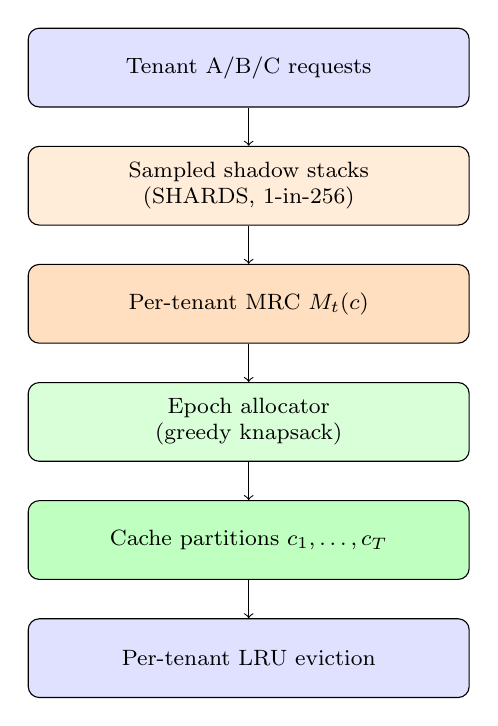
\begin{tikzpicture}[every node/.style={font=\footnotesize}]
  \tikzstyle{box}=[draw,rounded corners,minimum width=5.6cm,minimum height=1cm,align=center,inner sep=4pt]
  \node[box,fill=blue!12]   (tenants) at (0,7.5) {Tenant A/B/C requests};
  \node[box,fill=orange!15] (shard)   at (0,6.0) {Sampled shadow stacks\\(SHARDS, 1-in-256)};
  \node[box,fill=orange!25] (mrc)     at (0,4.5) {Per-tenant MRC $M_t(c)$};
  \node[box,fill=green!15]  (alloc)   at (0,3.0) {Epoch allocator\\(greedy knapsack)};
  \node[box,fill=green!25]  (parts)   at (0,1.5) {Cache partitions $c_1,\dots,c_T$};
  \node[box,fill=blue!12]   (lru)     at (0,0)   {Per-tenant LRU eviction};
  \draw[->] (tenants) -- (shard);
  \draw[->] (shard) -- (mrc);
  \draw[->] (mrc) -- (alloc);
  \draw[->] (alloc) -- (parts);
  \draw[->] (parts) -- (lru);
\end{tikzpicture}
\end{center}
\begin{center}\footnotesize Figure 1: request path, top to bottom. Sampling
and allocation run off the hot path; only eviction order is enforced per
access.\end{center}
\medskip

\Section{Evaluation Setup}
We replay three anonymised production traces (Prod-A/B/C) through a
trace-driven simulator that reproduces our production cache's eviction
semantics exactly, rather than benchmarking a live cluster — this lets us
compare policies on identical request sequences, which a live A/B test
cannot guarantee under shifting load. Each trace covers a 7-day window at
native request rate, replayed at $10\times$ speed. We compare
\textsc{TenantLRU} against three baselines: a single global LRU, static
per-tenant partitioning sized to each tenant's average working set, and an
oracle that knows each tenant's future access pattern in advance (an upper
bound, not a deployable policy).

\Section{Latency Over Time}
\begin{center}
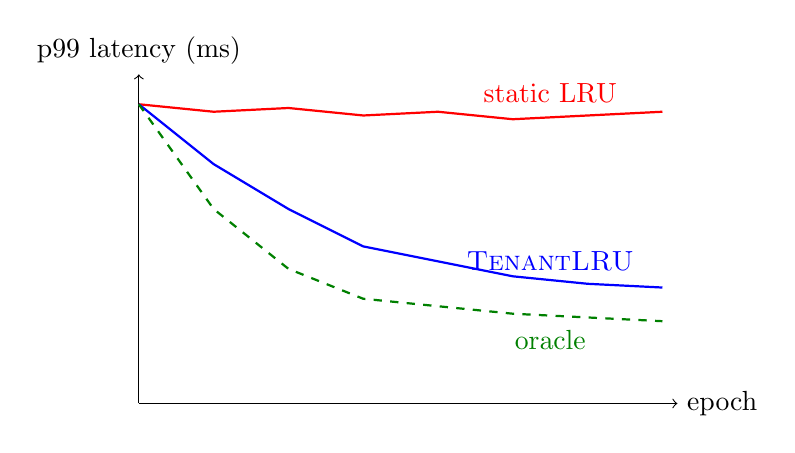
\begin{tikzpicture}[scale=0.95]
  \draw[->] (0,0) -- (7.2,0) node[right] {epoch};
  \draw[->] (0,0) -- (0,4.4) node[above] {p99 latency (ms)};
  \draw[thick,red] (0,4.0) -- (1,3.9) -- (2,3.95) -- (3,3.85) -- (4,3.9) -- (5,3.8) -- (6,3.85) -- (7,3.9);
  \draw[thick,blue] (0,4.0) -- (1,3.2) -- (2,2.6) -- (3,2.1) -- (4,1.9) -- (5,1.7) -- (6,1.6) -- (7,1.55);
  \draw[thick,green!50!black,dashed] (0,4.0) -- (1,2.6) -- (2,1.8) -- (3,1.4) -- (4,1.3) -- (5,1.2) -- (6,1.15) -- (7,1.1);
  \node[red] at (5.5,4.15) {static LRU};
  \node[blue] at (5.5,1.9) {\textsc{TenantLRU}};
  \node[green!50!black] at (5.5,0.85) {oracle};
\end{tikzpicture}
\end{center}
\begin{center}\footnotesize Figure 2: p99 latency converges within 4 epochs under
\textsc{TenantLRU}, closing most of the gap to the oracle upper bound.\end{center}
\medskip

\Section{Results}
\begin{center}
\begin{tabular}{lccc}
\toprule
Trace & Tenants & p50 $\downarrow$ & p99 $\downarrow$ \\
\midrule
Prod-A & 48 & 9\% & 38\% \\
Prod-B & 112 & 14\% & 41\% \\
Prod-C & 27 & 11\% & 44\% \\
\bottomrule
\end{tabular}
\end{center}
\begin{center}\footnotesize Table 1: Latency reduction vs.\ static LRU, three production traces.\end{center}
\medskip

\Section{Ablations}
\begin{center}
\begin{tabular}{lc}
\toprule
Variant & p99 vs.\ full system \\
\midrule
No SLA weighting ($w_t \equiv 1$) & $+9\%$ \\
No rebalance-rate cap & $+14\%$ \\
Continuous (no epochs) & $-2\%$, $6.1\times$ CPU \\
\bottomrule
\end{tabular}
\end{center}
\begin{center}\footnotesize Table 2: removing SLA weighting or the rebalance cap regresses
tail latency; running continuously barely helps but costs far more CPU.\end{center}
\medskip

The continuous variant confirms our epoch-based design does not leave much
latency on the table: solving the allocation problem on every access
recovers only 2\% further p99 improvement, at over $6\times$ the CPU cost
of the epoch-based scheme, which is not a trade we would make in
production.

\Section{Conclusions}
Per-tenant weighted allocation, driven by a cheap online miss-rate
estimate, closes most of the gap to an oracle partitioning scheme without
any offline tuning. Ongoing work extends the allocator to hierarchical
tenant groups and to write-heavy workloads where shadow-stack sampling is
more expensive.

\Section{References}
\begin{footnotesize}
\begin{enumerate}
\item Megiddo, N. and Modha, D.\ S.\ ARC: A Self-Tuning, Low Overhead Replacement Cache. \textit{FAST} 2003.
\item Beckmann, N.\ et al.\ LHD: Improving Cache Hit Rate by Maximizing Hit Density. \textit{NSDI} 2018.
\item Waldspurger, C.\ A.\ et al.\ Efficient MRC Construction with SHARDS. \textit{FAST} 2015.
\item Berger, D.\ S.\ et al.\ RobinHood: Tail Latency-Aware Caching --- Dynamic Reallocation from Cache-Rich to Cache-Poor. \textit{OSDI} 2018.
\item Ghandeharizadeh, S.\ et al.\ CAMP: A Cost Adaptive Multi-Queue Eviction Policy for Key-Value Stores. \textit{Middleware} 2020.
\end{enumerate}
\end{footnotesize}

\Section{Acknowledgements}
\begin{footnotesize}
We thank the Data Systems Lab infrastructure team for production trace
access, and our SIGMOD shepherd for detailed feedback on an earlier draft
of this work.
\end{footnotesize}

\end{multicols}
\end{document}
